% Authors:
% Bryan Consuegra, Panther ID 6040474
% Jessela Baniqued, Panther ID 6155725
% Leonardo Gutierrez, Panther ID 5105116 

\documentclass[twocolumn]{article}
\usepackage{amssymb}
\usepackage{graphicx}
\usepackage{array}
\usepackage{caption}
\usepackage{float}

\setlength{\parindent}{0pt}
\newcommand{\forceindent}{\leavevmode{\parindent=2em\indent}}

\title{A Survey of Perceived Aesthetics and Data Visualization Techniques}
\author{Bryan Consuegra\\Florida International University \and Jessela Baniqued\\Florida International University \and Leonardo Gutierrez \\Florida International University}
\date{4/12/20}

\begin{document}
	
	\maketitle
	
	\begin{abstract}
		%Here we describe the latest results on ...\\
		
		\forceindent This paper summarizes the research of Cawthon and Moere \cite{1} on the correlation between aesthetics, efficiency, and user engagement within the field of data visualization. In their paper, the duo conducted a study meant to quantify this correlation by using an online survey that revolved around the perceived aesthetics, data retrieval effectiveness, and engagement times with 11 different data visualization techniques. All visualizations represented the same data and were aesthetically normalized as much as possible while maintaining the predefined traits of any given visualization technique. The results of this study showed a direct correlation between user engagement and perceived aesthetics of a data visualization, as well as mixed results in identifying a relationship between data retrieval effectiveness and perceived aesthetics. These results may have been influenced by the color choice shared by the visualizations and the static presentation of some visualizations which benefit from interactivity in three dimensional space. \\
		
		{\bf Keywords}  data visualization, aesthetics, survey paper, human factors, user perception
	\end{abstract}

	\section{Introduction}	
		%Data Viz has recently made impressive advances in the area of graph drawing. Early discussions on the subject can be found in \cite{gpri_grapg_drawing} and \cite{rw_gs}. 
		
		\forceindent In a general sense, aesthetics can be defined as a branch of philosophy that studies the perception of beauty \cite{2}. While the philosophy of beauty may not be a core focus in the study of data visualization, there is still a discussion to be had on the effects of aesthetics on such a visual field of study. The use of aesthetics has been studied and applied in a number of different fields, such as user experience and product design, to stimulate specific positive reactions within a user or audience. In relation to data visualization, these positive reactions from users may translate to a longer engagement period with a visualization as well as a more complete and thorough understanding of the data being communicated through a visualization. Unfortunately, a lack of research in the relation between aesthetics and data visualization means that the correlation between aesthetics and data visualization remains a mostly hypothetical relation drawn from the research done in other less data-focused visual fields.
				
		\forceindent On the other hand, the lack of research within the topic of aesthetics in data visualization has left the door open for researchers to become pioneers in such research. Cawthon and Moere \cite{1} have made themselves known as two such pioneers with their study on "The Effect of Aesthetic on the Usability of Data Visualization." Their study had made some impressive findings in several relationships that exist between users, aesthetics, and data visualization. This paper aims to summarize this study and its findings, as well as areas of improvement can be addressed in future studies of aesthetics and data visualizations.
		
	\section{Survey}
	\forceindent This section goes over Cawthon and Moere's study by summarizing the parameters and potential relations tested for in the study, followed by the methodology of the study, the results of the study, and any factors that may have influenced the study's results.
	
		\subsection{Parameters Measured}
		
		\forceindent This study attempts to quantify the relationship between aesthetics and the "usability of data visualization" by using different measures of effectiveness, efficiency, task abandonment, and user patience. Effectiveness in this study is defined by how accurately a user is able to analyze information from a data visualization, and efficiency is defined by how quickly a user is able to analyze information correctly from a data visualization. Task abandonment is defined as when a user abandons an attempt to analyze information from a data visualization, usually due to too much information (either visual information or data) being presented. Additionally, user patience is measured using two different values: erroneous response latency and abandonment response latency. These two values indicate the amount of time a user is willing to invest in analyzing a data visualization before coming to an erroneous analysis of the data and abandoning analysis of the data, respectively. Finally, rankings and scales are used to quantify the perceived aesthetics of a visualization, or how aesthetic pleasing or displeasing a visualization appears to a user.
		
		\subsection{Methodology}
		
		\forceindent The study was conducted using an online survey that was accessed by 285 participants, all of whom were recruited through various online forums and postings. Participants came from a variety of backgrounds and nationalities, but many participants shared some formal background in design—mostly due to the survey being shared heavily among information architecture and design forums. The online survey taken by participants gives a subset of 7 data visualizations from a total set of 11 data visualizations and asks participants to answer a series of questions based on those 7 visualizations. All 11 data visualizations represent the same data (a hierarchical representation of a file directory), and all data visualizations were normalized as much as possible in regards to color, size/scale of the visual, and typography. The same color palette of 11 earth-toned colors were used in each visualization that required coloring, and all visualizations were presented in the same size, scale, positioning, and all used the same typography. The types of questions asked in the survey can be split into two sections: "aesthetic ranking" and "task performance." 
		
		\forceindent Firstly, the aesthetic ranking section asked participants to rate the aesthetic appeal of a series of visualizations "as they 'would with a painting or illustration'". Participants were asked to rank each of the 7 visualizations individually using a slider bar with values ranging from "ugly" to "beautiful." Participants were then asked to rank the aesthetic appeal of each visualization relative to the other visualizations, placing each visualization on a ranking tier list from "ugly" to "beautiful." Afterwards, the task performance section of the survey asked participants 14 randomly selected structure and attribute-related questions of the subset of 7 data visualizations, 2 questions per visualization. Each question was designed to be answered by having the user analyze and retrieve data from the visualization. Each question gave 6 multiple-choice options, including 1 "cannot tell" option on each question. The "cannot tell" option is equivalent to the user abandoning the task of data retrieval. During each of the 14 questions, the participants are timed from when the question is first displayed to when the participant selects a response, and those times are recorded along with participants' answers. Effectiveness is measured by a participant's rate of correct responses (the percentage of questions they answer correctly out of the 14 questions), and efficiency is measured by the time it takes for a participant to answer a question correctly, in seconds. Task abandonment is measured by a participant's rate of abandonment, or the number of questions in which the participant answered "Cannot tell." Finally, erroneous response latency is measured by a participant's error response time, or how much time a user invests in a problem before giving an incorrect answer, and abandonment response latency is measured by a participant's abandonment response time, or how much time a user invests in a problem before giving "Cannot tell" as an answer.

		\subsection{Results}\forceindent This subsection discusses the different measurements and findings found in the study's results.
		
		\subsubsection{Perceived Aesthetics}
		\forceindent The rankings used by participants to rate the aesthetic qualities of a visualization were quantified on a scale from 0 to 100, with 0 being as "ugly" as possible and 100 being as "beautiful" as possible. The SunBurst data visualization was rated the highest with an average rating of 58 in individual rankings and 69 in group rankings, and  the BeamTrees data visualization was rated the lowest with an average rating of 36 in individual rankings and 32 in group rankings. Most visualizations were rated higher in group rankings than individuals rankings, which the authors attribute to design differences in the group rankings section of the survey; for example, allowing the ratings of different visualizations to overlap. Otherwise, there appeared to be no trends in the aesthetic rankings that would suggest any key design feature influencing a visualization's perceived aesthetics. For instance, the three three-dimensional visualizations all had significantly different rankings, and the two similar visualizations TreeMap and IcicleTree were also ranked significantly differently.
		
		\subsubsection{Measures of Usability}
		\forceindent In terms of effectiveness, all three of the three-dimensional visualizations were found to be part of the four least effective visualizations. Botanical Viewer, StepTree, and BeamTrees had rates of correct responses of 43\%, 42\%, and 28\%, respectively. The only two-dimensional visualization that ranked lower than any three-dimensional visualizations was the TreeMap visualization, with a correct response rate of 32\%. Similar to their effectiveness, the Botanical Viewer and StepTree visualizations were the two least efficient visualizations with correct response times of 39.6 and 39.0 seconds, respectively. While the BeamTrees visualization was ranked as the least aesthetically pleasing visualization, the results showed the visualization to have an average effectiveness and efficiency level, outranking the other three-dimensional visualizations. The color-coded IcicleTree visualization was shown to be 7\% more effective and 2.5 seconds more efficient than the Dendogram Tree visualization, which features a very similar structure without the use of color-coding. \\ \\
		\forceindent As for latency in error responses, it was generally found that participants were willing to invest more time analyzing a visual that ranked highly in aesthetics. For example, the SunBurst visualization, which ranked the highest on the perceived aesthetics rankings, had the longest erroneous response times at 47.1 seconds. On the other hand, the BeamTrees visualization, which ranked the lowest on the perceived aesthetics rankings, had the shortest erroneous response times at 35.6 seconds. The rate of abandonment is somewhat inverse to the rate of correct responses (or effectiveness), in that visualizations with high correct response rates have low abandonment rates, and vice versa.  However, the task abandonment response time of different visualizations had a lot of variation that appeared independent of perceived aesthetics, effectiveness and efficiency.
		
		\subsubsection{Data}
		
		\begin{table}[H]
			{\renewcommand{\arraystretch}{1.4}
				\begin{tabular}{|r*{5}{|m{.6cm}}|}
					\cline{2-6}
					\multicolumn{1}{c|}{} & \textbf{\rotatebox[origin=c]{90}{\parbox[c]{5cm}{ Rate of Correct \\ Response (\%) }}} & \textbf{\rotatebox[origin=c]{90}{\parbox[c]{5cm}{ Correct Response \\ Time (seconds) }}} & \textbf{\rotatebox[origin=c]{90}{\parbox[c]{5cm}{ Error Response \\ Time (seconds) }}} & \textbf{\rotatebox[origin=c]{90}{\parbox[c]{5cm}{ Rate of \\ Abandonment (\%)}}} & \textbf{\rotatebox[origin=c]{90}{\parbox[c]{5cm}{ Abandonment Response \\ Time (seconds) }}}\\
					\hline
					\textit{TreeMap} &  .32 & 35.0 & 37.3 & .38 & 34.5 \\
					\hline
					\textit{Botan.Viewer} & .43 & 39.6 & 40.6 & .32 & 35.3 \\
					\hline
					\textit{SunBurst} & .84 & 23.2 & 47.1 & .07 & 37.8 \\
					\hline
					\textit{IcicleTree } & .81 & 22.0 & 41.2 & .12 & 42.4 \\
					\hline
					\textit{SpaceTree} & .73 & 20.8 & 40.9 & .06 & 52.1 \\
					\hline
					\textit{Win. Explorer} & .79 & 21.8 & 38.0 & .08 & 38.6 \\
					\hline
					\textit{BeamTree} & .28 & 27.7 & 35.6 & .55 & 29.9 \\
					\hline
					\textit{StarTree} & .81 & 23.4 & 43.5 & .07 & 50.8 \\
					\hline
					\textit{Dendo.Tree} & .74 & 25.7 & 43.2 & .11 & 43.2 \\
					\hline
					\textit{Polar View} & .69 & 27.6 & 37.2 & .15 & 35.0 \\
					\hline
					\textit{StepTree} & .42 & 39.0 & 40.6 & .35 & 29.6 \\
					\hline
			\end{tabular}}\\\\
			\caption{Measures of effectiveness, efficiency, erroneous response, and task abandonment.}
		\end{table}
		
		\subsubsection{Visualizations}
		
		\begin{figure}[H]
			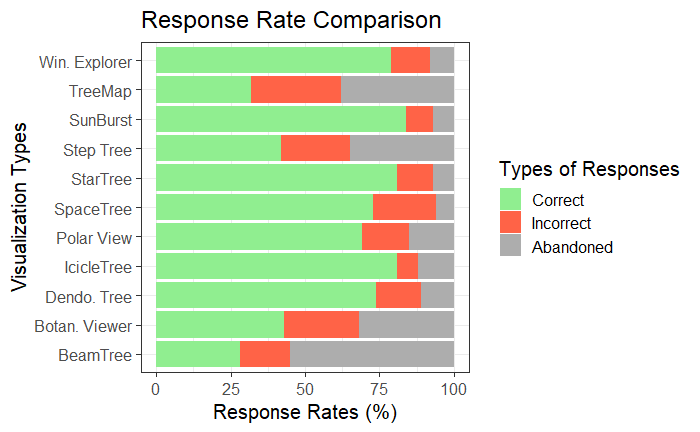
\includegraphics[scale=0.57]{response_rate_comparison.png}
			\caption{Response Rate Comparison}
			\label{Response Rate Comparison}
		\end{figure}
		\begin{figure}[H]
			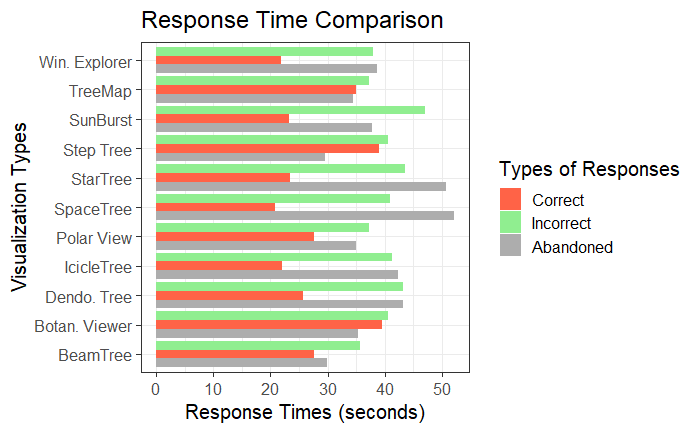
\includegraphics[scale=0.57]{response_time_comparison.png}
			\caption{Response Time Comparison}
			\label{Response Time Comparison}
		\end{figure}
	
		Figure \ref{Response Rate Comparison} and Figure \ref{Response Time Comparison} compare all the techniques on three cases. Figure \ref{Response Rate Comparison} compares the rate at which	individuals responded correctly, incorrectly, or abandoned. Figure \ref{Response Time Comparison} compares how long it took them to reach that conclusion in the same three cases.
\\
		
		\begin{figure}[H]
			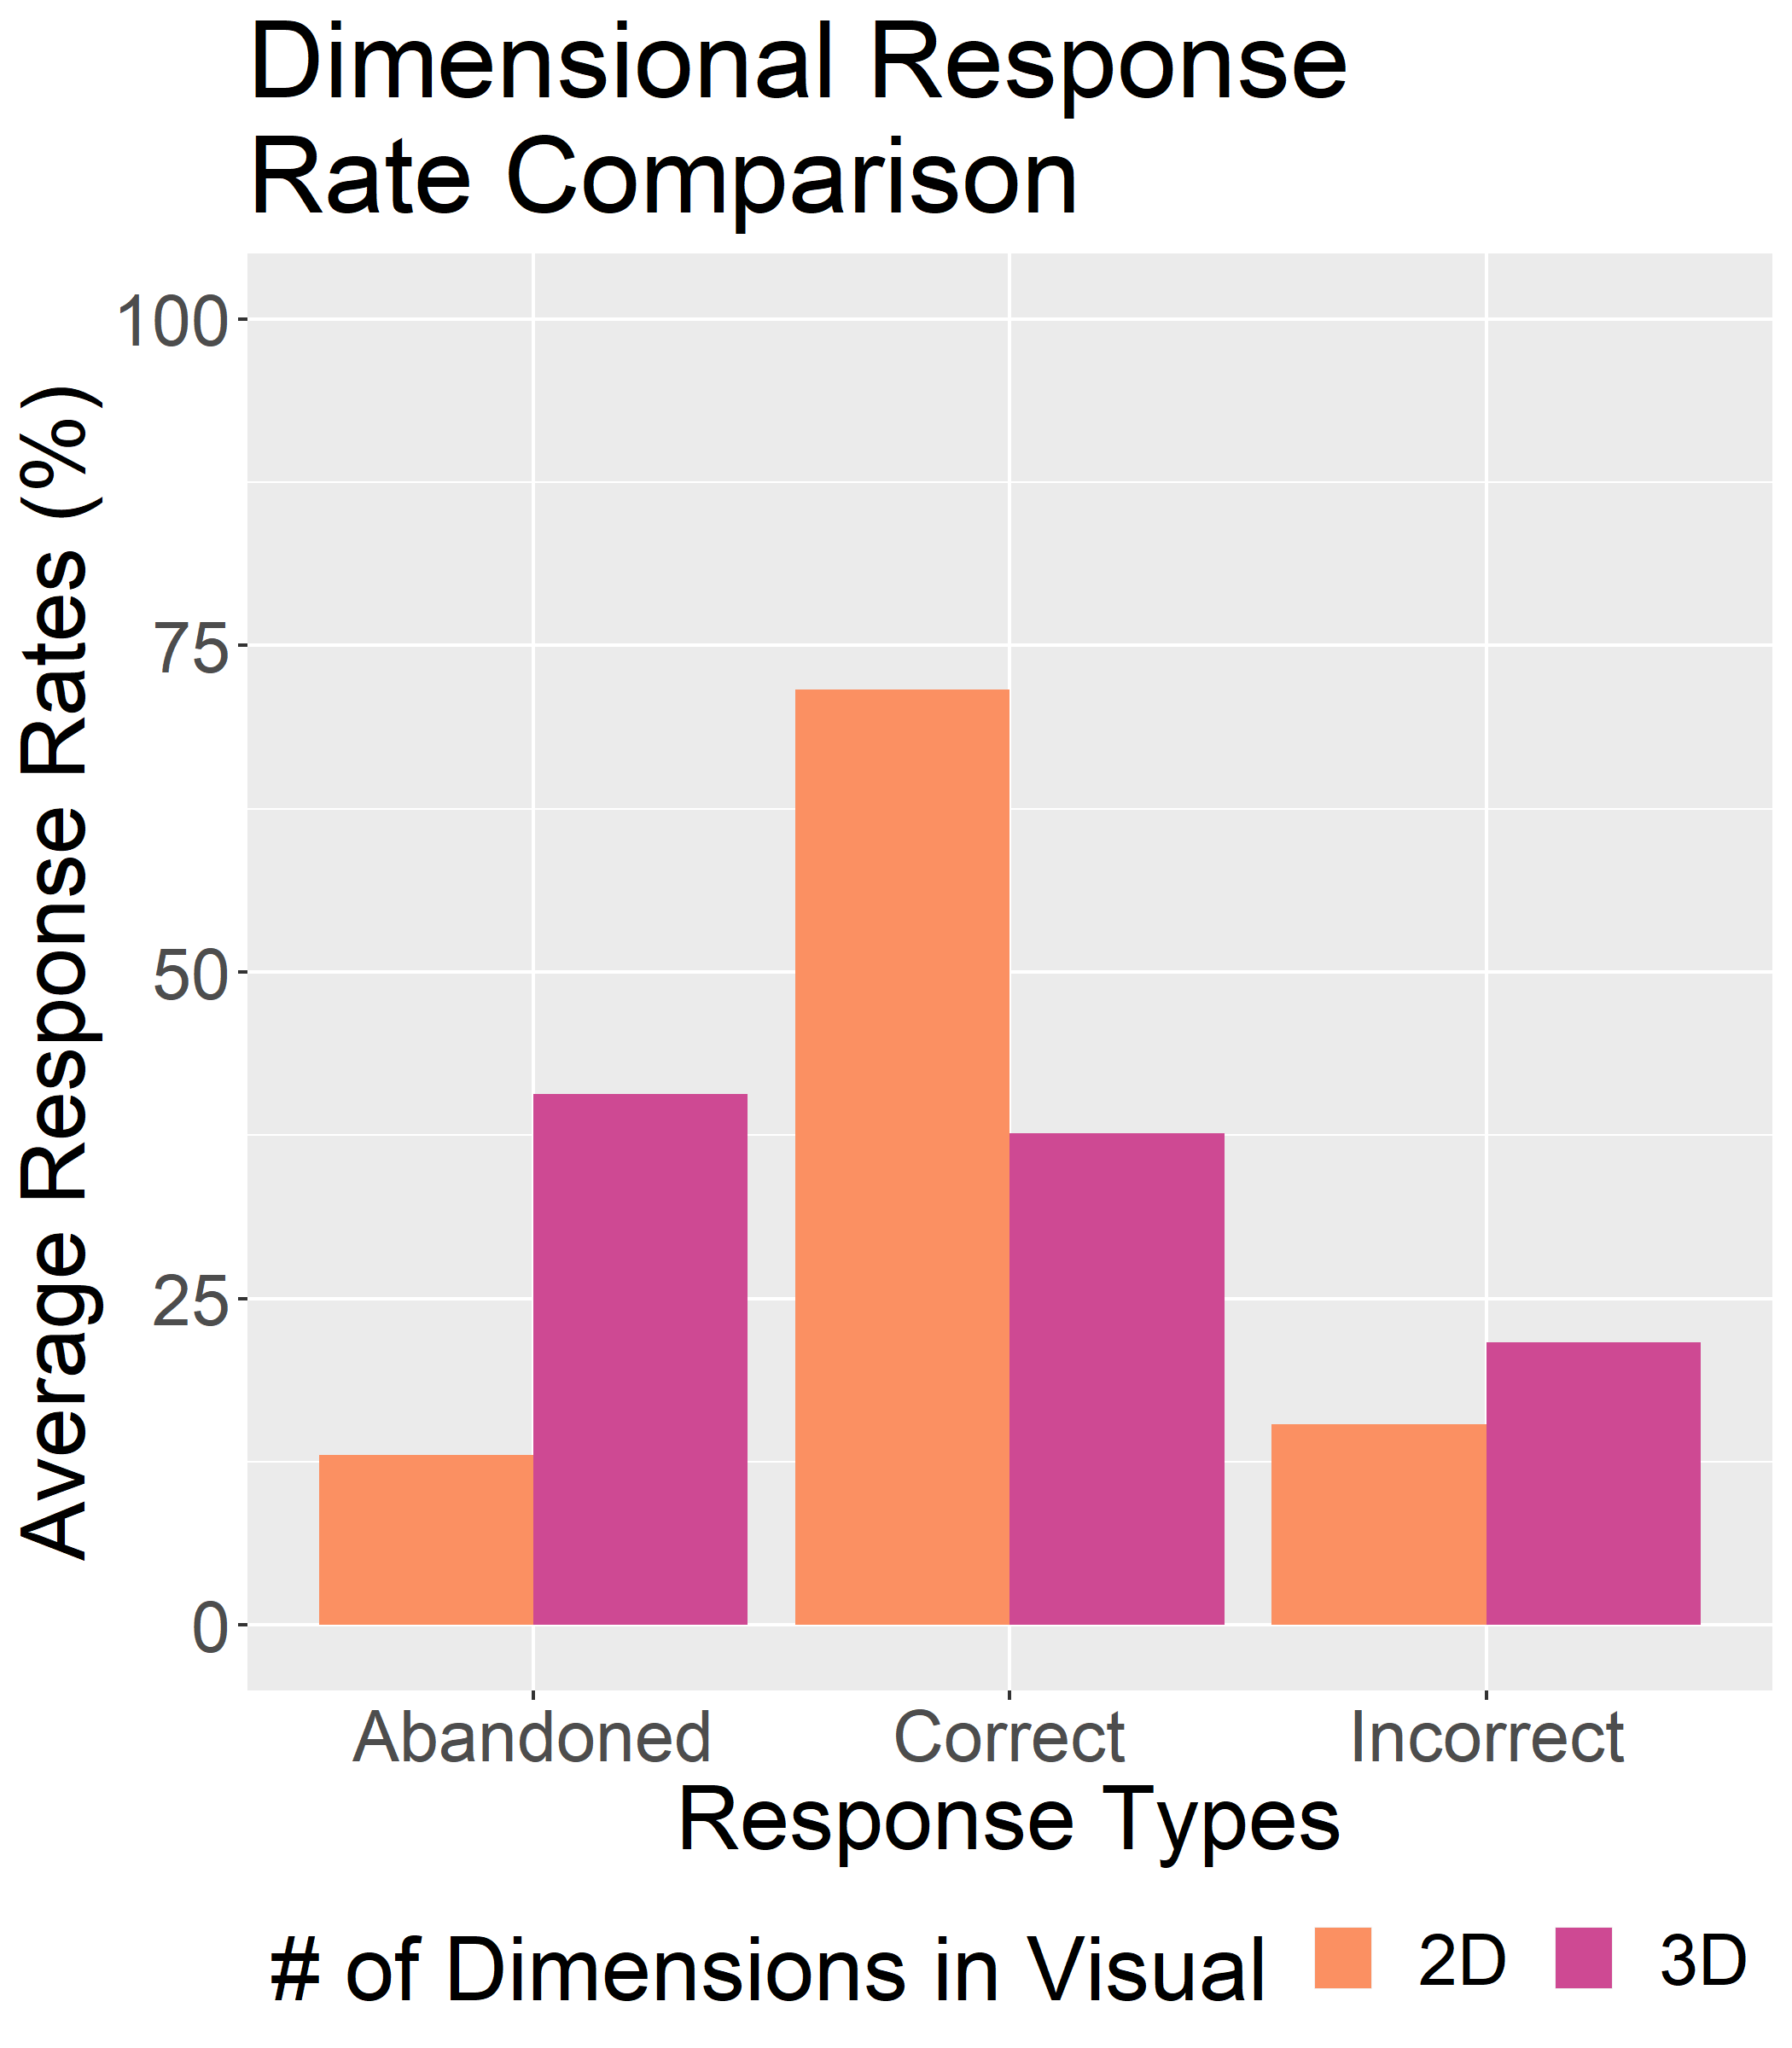
\includegraphics[scale=0.415]{response_rate_dimensional_comparison.png}
			\caption{Response Rate Dimensional Comparison}
			\label{Response Rate Dimensional Comparison}
		\end{figure}
		\begin{figure}[H]
			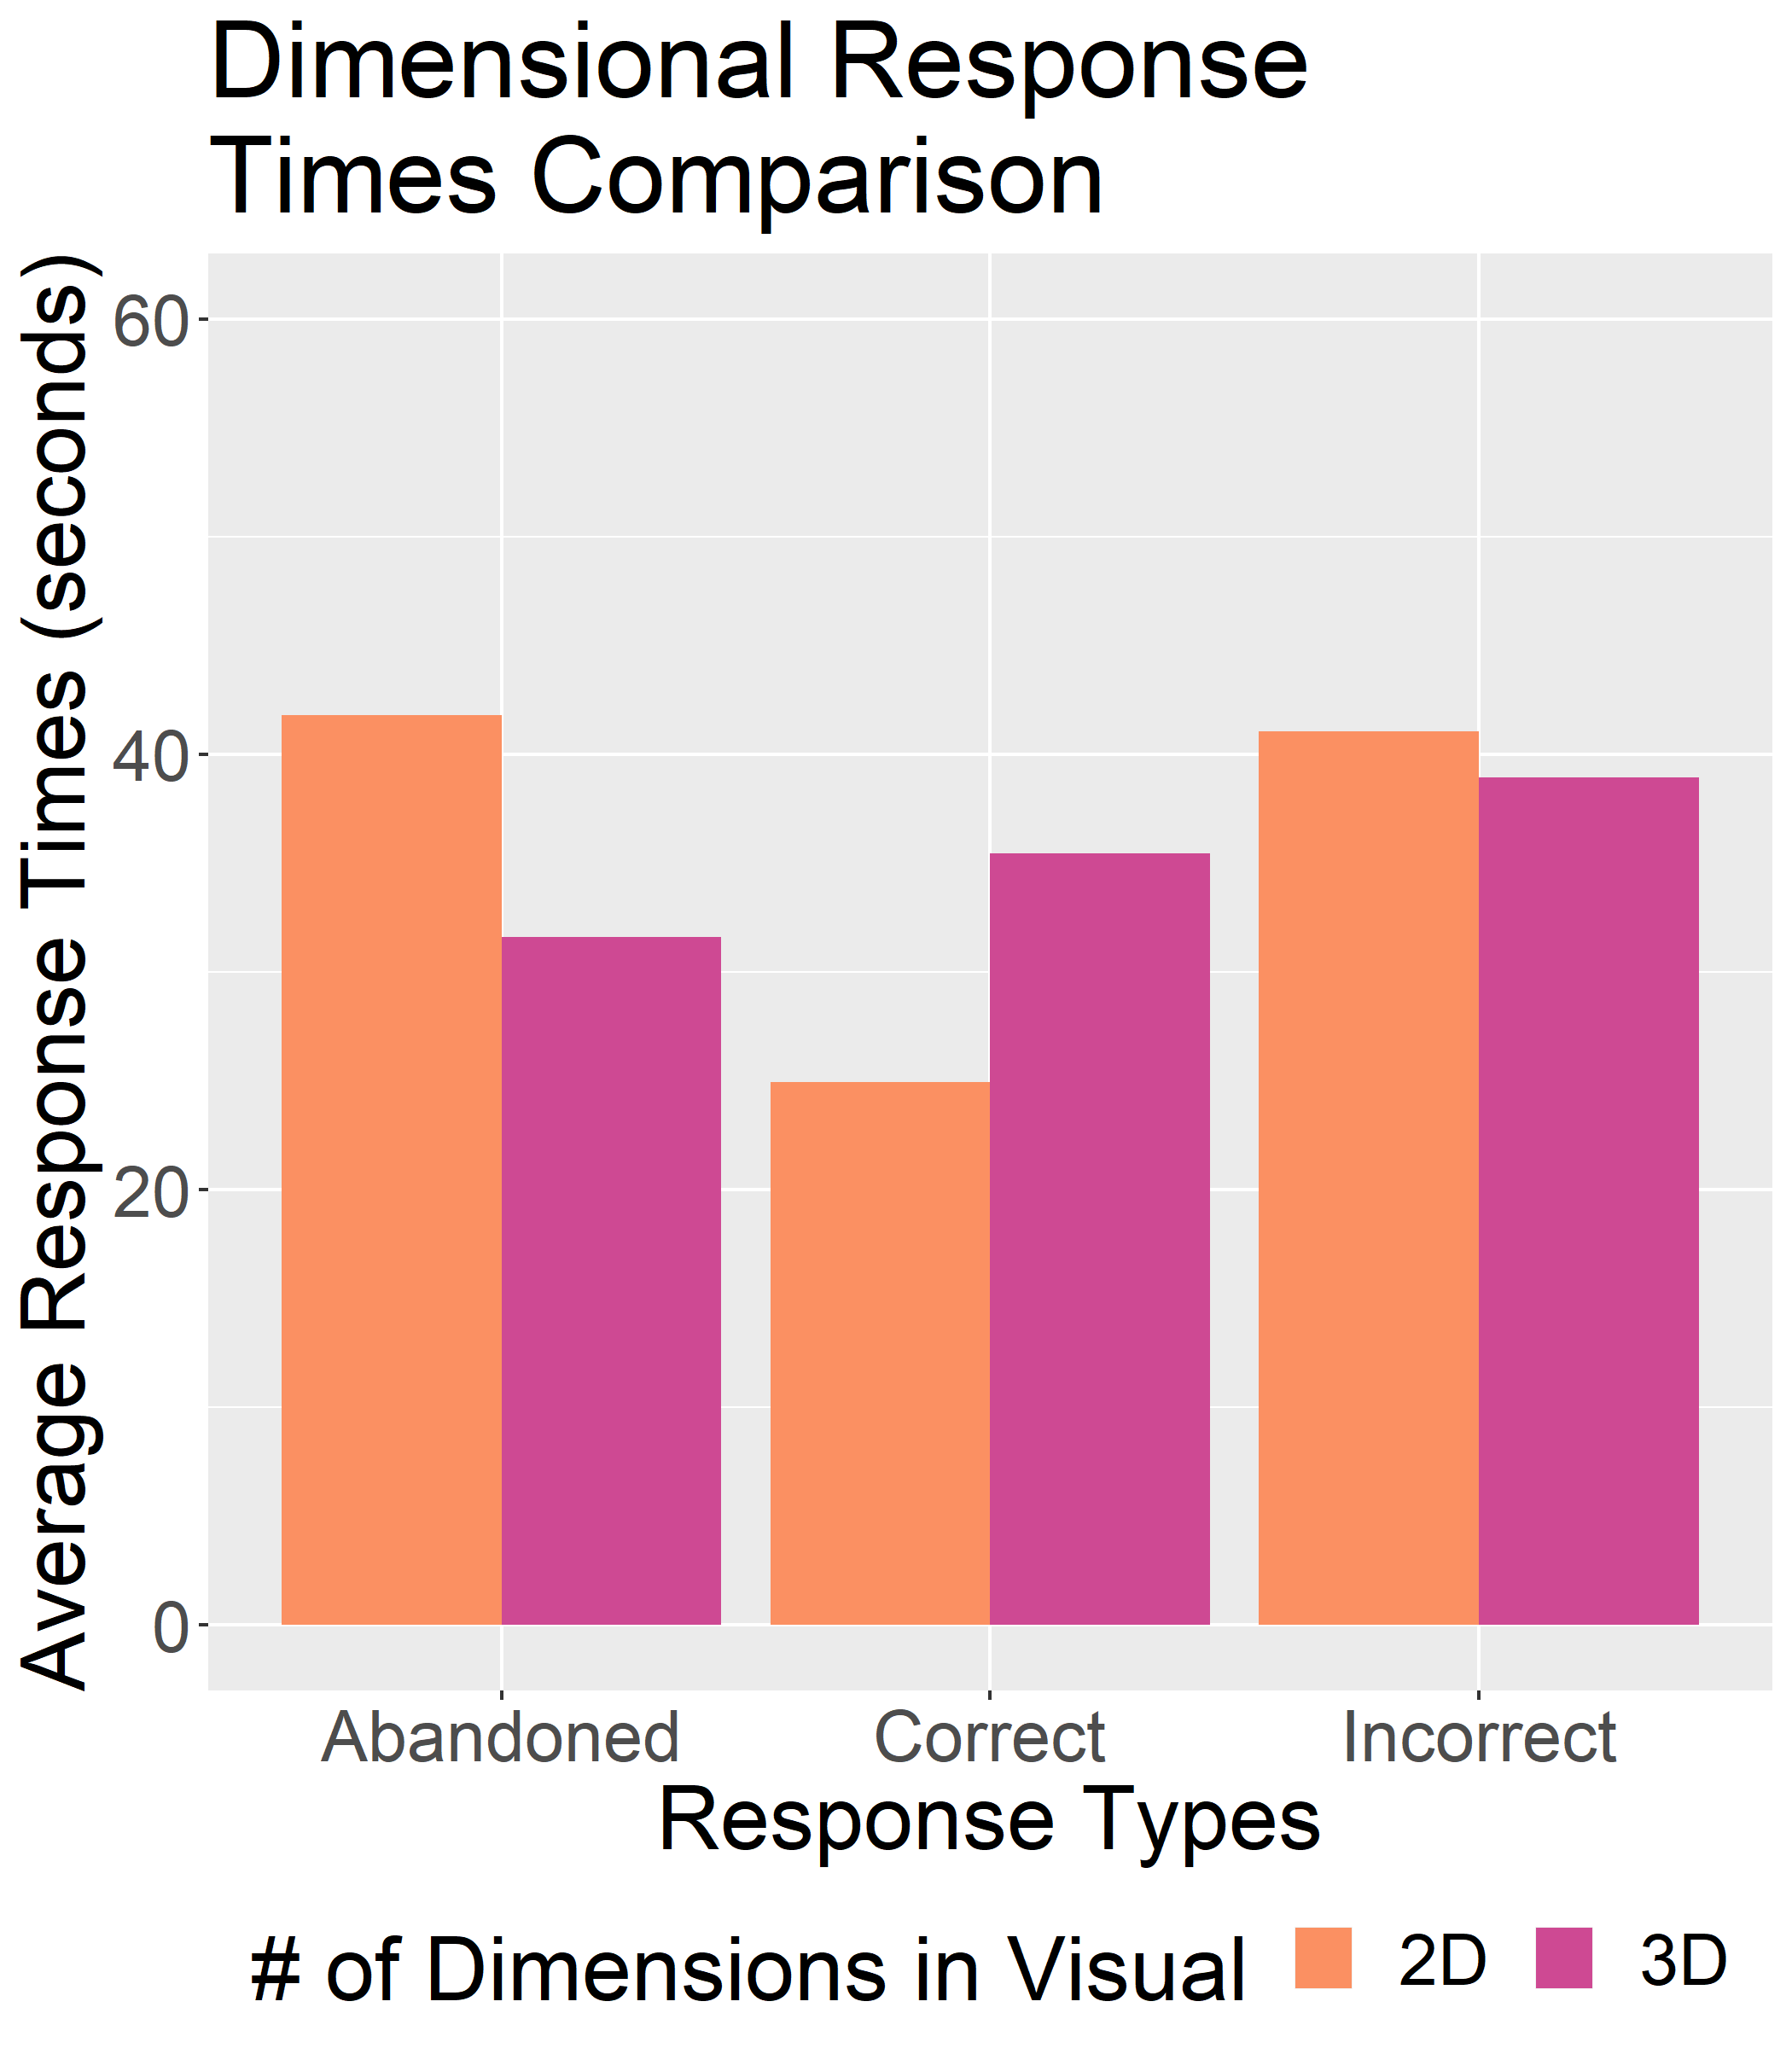
\includegraphics[scale=0.415]{response_time_dimensional_comparison.png}
			\caption{Response Time Dimensional Comparison}
			\label{Response Time Dimensional Comparison}
		\end{figure}
	
		Figure \ref{Response Rate Dimensional Comparison} and Figure \ref{Response Time Dimensional Comparison} compare the effectiveness of 2D techniques and 3D techniques. For each of the cases (correct, incorrect, and abandoned), the average performance is shown.\\

		\subsection{Analysis}
		
		\forceindent While the results of this study did indicate some clear correlations between aesthetics and the usability of data visualization, the results also provide some muddled results on other possible correlations.
		
		\forceindent For instance, the SunBurst and BeamTree visualizations, who ranked as the most and least aesthetically pleasing visualizations, respectively, were also the most and least effective visualizations, respectively. Moreover, SunBurst was also the most efficient visualization and the visualization with the second lowest task abandonment rate, while BeamTree had the highest task abandonment rate. These results suggest correlation between perceived aesthetics and effectiveness/efficiency. However, other visualizations with lower rankings in perceived aesthetics, such as Windows Explorer and SpaceTree, were some of the most effective and most efficient data visualizations, going against the proposed correlation between aesthetics and effectiveness/efficiency.
		
		\forceindent A clearer correlation can be found between the use of two-dimensional space or three-dimensional space in a visualization and the effectiveness of that visualization. As discussed in the Results subsection of this survey, the three three-dimensional data visualizations (Botanical Viewer, StepTree, and BeamTrees) made up three of the four least effective visualizations. On average, three-dimensional visualizations were found to be far less effective than two-dimensional visualizations. However, this decrease in effectiveness may have been caused by the use of static images to present the three-dimensional visualizations to participants taking the online survey. Cawthon and Moere hypothesize that the three-dimensional visualizations would have been more effective if they were able to be presented in the dynamic and interactable environments that the three-dimensional visualizations were originally designed for.
		
		\forceindent While there appeared to be no discernible correlation between color and usability of a visualization, Cawthon and Moere also propose that the use of a different color palette throughout all the visualizations may have affected the overall results of the study, depending on color theory and whether the palette used facilitates information acquisition for the human eye.
		
		\forceindent The data visualizations ranking at 70\% correct response rates or above all shared a few similarities that could highlight what participants look for in an effective data visualization. These include easy to identify elements, usually clearly color-coded, and easy to identify relationships between elements (especially since the data in this study was a hierarchical dataset). These highly effective data visualizations also avoided the use of 3-D visuals in their static image form, reducing the complexity of the visualizations.
		
	\section{Conclusions}
	
	\forceindent The results found in Cawthon and Moere's study on aesthetics and usability of data in data visualizations suggest that aesthetics do play some part in the effectiveness and efficiency of a data visualization, although visualizations that are not necessarily aesthetically pleasing can be effective/efficient as long as they have clearly defined elements and relations between elements.
	
	\forceindent Other correlations between aspects of aesthetics, such as color and structure, and other measurements of data usability, such as rate of erroneous responses and abandonment response time, cannot be definitively drawn without further research. The field of data visualizations would benefit from using the study of Cawthon and Moere as a springboard to launch more findings to more accurately analyze correlations between aesthetics and data usability.
	

	\bibliographystyle{plain}
	\bibliography{graphviz}
	
\end{document}